\begin{surferPage}[Kummer-Quartic]{Kummer Quartic}
		Eduard Kummer je bio prvi koji je 1875.\ godine postavio pitanje koliki je najve\' ci broj singulariteta $\mu(d)$ na plohi stupnja $d$. U njegovom slu\v caju, stupanj plohe je bio $4$, a svaku takvu plohu stupnja $4$ zovemo \emph{quartic}.
		
Kummer je otkrio da je $\mu(4)=16$. Nakon toga je detaljnije prou\v cavao plohe quartic sa $16$ singulariteta.
Posebno lijepa familija takvih ploha je odre\dj ena sa:
\[\bigl(x^2+y^2+z^2-\mu^2\bigr)^2 - \lambda
\,y_0\,y_1\,y_2\,y_3,\]
gdje je $\mu$ slobodan parametar, a 
$\lambda = \frac{3\mu^2-1}{3-\mu^2}$, dok su $y_i$ strane pravilnog 
tetraedra {\small
    $y_0=1-z-\sqrt{2}x$, \  
    $y_1=1-z+\sqrt{2}x$, \ 
    $y_2=1+z+\sqrt{2}y$, \ 
    $y_3=1+z-\sqrt{2}y$},
	kako bi ploha bila simetri\v cna.
	Nemaju sve plohe iz ove familije ploha to\v cno $16$ realnih singulariteta, iako ve\' cina njih ima to svojstvo:
	\begin{center}
    \vspace*{-0.2cm}\hspace*{-0.2cm}
    \begin{tabular}{@{}c@{\,}c@{\,}c@{\,}c@{\,}c@{}}
      \begin{tabular}{@{}c@{}}
        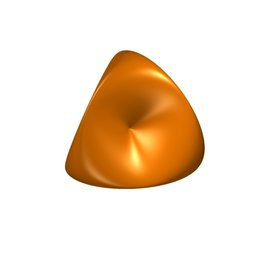
\includegraphics[height=1.4cm]{./../../common/images/kummer_0}
      \end{tabular}
      &
      \begin{tabular}{@{}c@{}}
        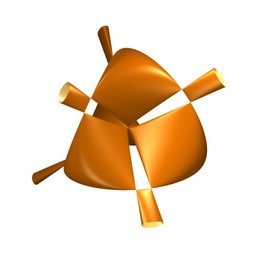
\includegraphics[height=1.4cm]{./../../common/images/kummer_1}
      \end{tabular}
      &
      \begin{tabular}{@{}c@{}}
        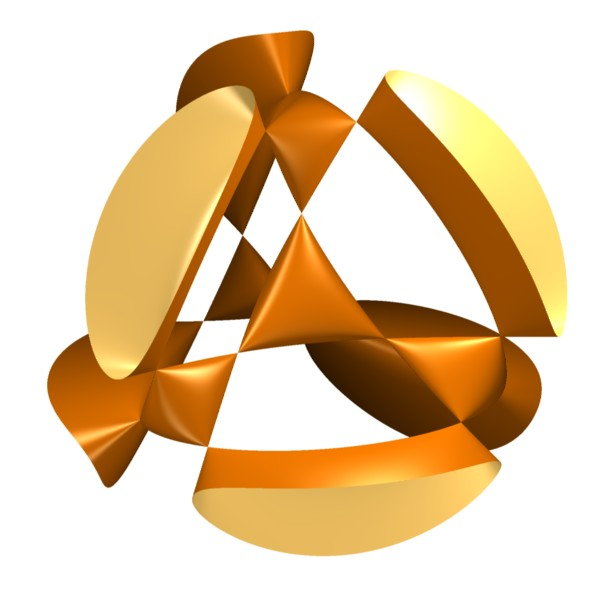
\includegraphics[height=1.4cm]{./../../common/images/kummer_2}
      \end{tabular}
      &
      \begin{tabular}{@{}c@{}}
        
\includegraphics[height=1.4cm]{./../../common/images/kummer_3}
      \end{tabular}
    \end{tabular}
  \end{center}
  \vspace{-0.2cm}
		Za neke posebne vrijednosti parametara, neki od singulariteta se mogu podudarati.
\end{surferPage}
